% !TEX root = ../thesis.tex
\graphicspath{{./vega-lite/figures/}}
\chapter{A Grammar of Interactive Graphics}
\label{sec:vega-lite}

\begin{figure}[h!]
  \vspace{-40pt}
  \centering
  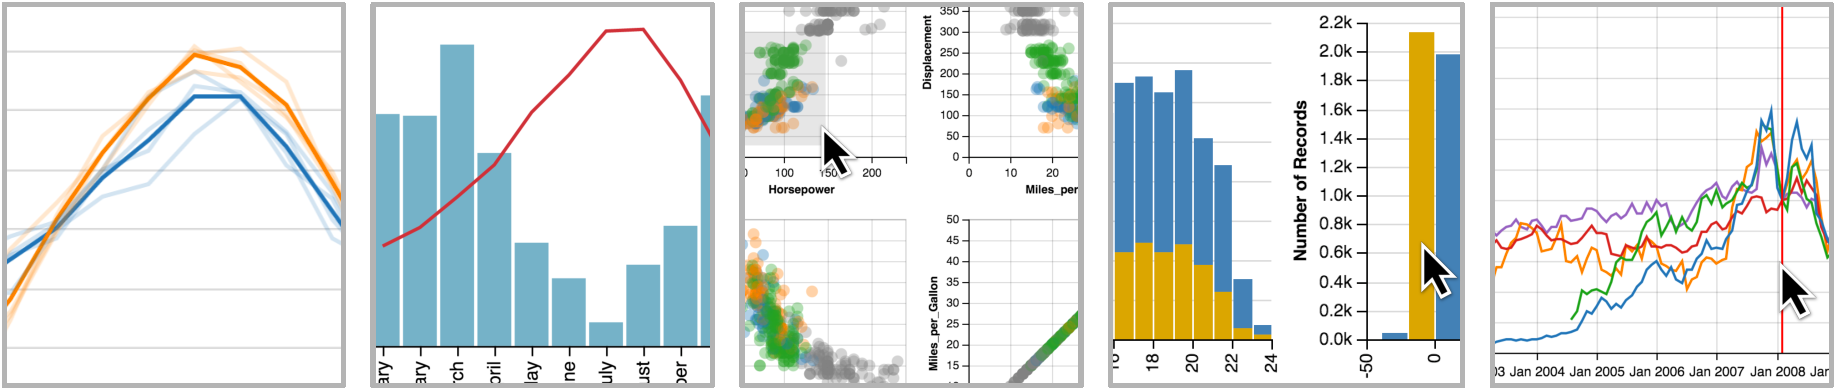
\includegraphics[width=0.9\columnwidth]{teaser}
  % \vspace{-30pt}
\end{figure}

% Reactive Vega demonstrates that the advantages of declarative specification
% extend to interaction design as well\,---\,decoupling specification from
% execution frees designers to iterate more quickly, facilitates retargeting
% across platforms, and allows for language-level optimizations.

Reactive Vega demonstrates that declarative interaction design is an expressive
and performant alternative to imperative event handling callbacks. However, as
its abstractions are relatively low-level, it is best described as an ``assembly
language'' for interactive visualization most suited for \emph{explanatory}
visualization. In contrast, for \emph{exploratory} visualization, higher-level
grammars such as ggplot2~\cite{wickham:layered}, and grammar-based systems such
as Tableau (n\'ee Polaris~\cite{stolte:polaris}), are typically preferred as
they favor conciseness over expressiveness. Analysts rapidly author partial
specifications of visualizations; the grammar applies default values to resolve
ambiguities, and synthesizes low-level details to produce visualizations.

High-level languages can also enable search and inference over the space of
visualizations. For example, Wongsuphasawat et~al. introduced Vega-Lite to power
the Voyager visualization browser~\cite{voyager}. With a smaller surface area
than Vega, Vega-Lite makes systematic enumeration and ranking of data
transformations and visual encodings more tractable.

However, existing high-level languages provide limited support for
interactivity. An analyst can, at most, enable a predefined set of common
techniques (linked selections, panning \& zooming, etc.) or parameterize their
visualization with dynamic query widgets~\cite{shiny}. For custom, direct
manipulation interaction they must turn to imperative event callbacks.

In this chapter, we extend Vega-Lite with a \emph{multi-view} grammar of
graphics and a \emph{grammar of interaction} to enable concise, high-level
specification of interactive data visualizations.

% !TEX root = ../thesis.tex
\section{Visual Encoding}
\label{sec:vlgog}

The simplest Vega-Lite specification\,---\,referred to as a \emph{unit}
specification\,---\,describes a single Cartesian plot with the following
four-tuple:

\signaturevspace
\centerline{\emph{unit := (data, transforms, mark-type, encodings)}}
\signaturevspace

The \emph{data} definition identifies a data source, a relational table
consisting of records (rows) with named attributes (columns). This data table
can be subject to a set of \emph{transforms}, including filtering and adding
derived fields via formulas. The \emph{mark-type} specifies the geometric object
used to visually encode the data records. Legal values include \emph{bar},
\emph{line}, \emph{area}, \emph{text}, \emph{rule} for reference lines, and
plotting symbols (\emph{point} \& \emph{tick}). The \emph{encodings} determine
how data attributes map to the properties of visual marks. Formally, an encoding
is a seven-tuple:

\signaturevspace
\centerline{\emph{encoding := (channel, field, data-type, value, functions, scale, guide)}}
\signaturevspace

Available visual encoding \emph{channels} include spatial position (\emph{x},
\emph{y}), \emph{color}, \emph{shape}, \emph{size}, and \emph{text}. An
\emph{order} channel controls sorting of stacked elements (e.g., for stacked bar
charts and the layering order of line charts). A \emph{path} order channel
determines the sequence in which points of a line or area mark are connected to
each other. A \emph{detail} channel includes additional group-by fields in
aggregate plots.

The \emph{field} string denotes a data attribute to visualize, along with a
given \emph{data-type} (one of \emph{nominal}, \emph{ordinal}, \emph{quantitative} or
\emph{temporal}). Alternatively, one can specify a constant literal \emph{value}
to serve as the data field. The data field can be further transformed using
\emph{functions} such as binning, aggregation (e.g., mean), and sorting.

An encoding may also specify properties of a \emph{scale} that maps from the
data domain to a visual range, and a \emph{guide} (axis or legend) for
visualizing the scale. If not specified, Vega-Lite will automatically populate
default properties based on the \emph{channel} and \emph{data-type}. For \emph
{x} and \emph{y} channels, either a linear scale (for quantitative data) or an
ordinal scale (for ordinal and nominal data) is instantiated, along with an
axis. For \emph{color}, \emph{size}, and \emph{shape} channels, suitable
palettes and legends are generated. For example, quantitative color encodings
use a single-hue luminance ramp, while nominal color encodings use a categorical
palette with varied hues. Our default assignments largely follow the model of
prior systems~\cite{stolte:polaris, voyager}.

Unit specifications are capable of expressing a variety of common, useful plots
of both raw and aggregated data. Examples include bar charts, histograms, dot
plots, scatter plots, line graphs, and area graphs. Our formal definitions are
instantiated in a JSON (JavaScript Object Notation) syntax, as shown in
% \fig{Units}.

\section{View Composition Algebra}

Multiple \emph{unit} specifications can be composed using the following
operators:

\begin{itemize}
  \item \emph{layer([$unit_1$, $unit_2$, ...], resolve)} produces a view in
  which subsequent charts are plotted on top of each other. To produce coherent
  and comparable layers, we share scales (if their types match) and merge guides
  by default. For example, we compute the union of the data domains for the
  \emph{x} or \emph{y} channel, for which we then generate a single scale.
  However, Vega-Lite can not enforce that a unioned domain is
  \emph{semantically} meaningful. To prohibit layering of composite views with
  incongruent internal structures, the \emph{layer} operator restricts its
  operands to be \emph{unit} views.

  \item \emph{hconcat([$view_1$, $view_2$, ...], resolve)} and
  \emph{vconcat([$view_1$, $view_2$, ...], resolve)} place views side-by-side
  horizontally or vertically, respectively. If aligned spatial channels have
  matching data fields (e.g., the \emph{y} channels in an \emph{hconcat} use the
  same field), a shared scale and axis are used. Axis composition facilitates
  comparison across views and optimizes the underlying implementation.

  \item \emph{facet(data, field, view, channel, scale, axis, resolve)} produces
  a trellis plot~\cite{becker:trellis} by subsetting the \emph{data} by the
  distinct values of a \emph{field}. The \emph{view} specification provides a
  template for the sub-plots, and inherits the backing \emph{data} for each
  partition from the operator. The \emph{channel} indicates if sub-plots should
  be laid out vertically (\emph{row}) or horizontally (\emph{column}), and the
  \emph{scale} and \emph{axis} parameters enable further customization of
  sub-plot layout and labeling.

    To facilitate comparison, scales and guides for quantitative fields are shared
  by default. This ensures that each facet visualizes the same data domain.
  However, for ordinal scales we generate independent scales by default to avoid
  unnecessary inclusion of empty categories, akin to Polaris' \emph{nest}
  operator. When faceting by fiscal quarter and visualizing per-month data in each
  cell, one likely wishes to see three months per quarter, not twelve months of
  which nine are empty.

  \item \emph{repeat(values, view, channel, scale, axis, resolve)} generates
  one plot for each entry in a list of \emph{values}. The \emph{view}
  specification provides a template for the sub-plots, and inherits the full
  backing dataset. Encodings within the repeated \emph{view} specification can
  refer to this provided \emph{value} to parameterize the plot\footnote{As the
  \emph{repeat} operator requires parameterization of the inner view, it is not
  strictly algebraic. It is possible to achieve algebraic ``purity'' via
  explicit repeated concatenation or by reformulating the repeat operator (e.g.,
  by including rewrite rules that apply to the inner view specification).
  However, we believe the current syntax to be more usable and concise than
  these alternatives.}. As with \emph{facet}, the \emph{channel} indicates if
  plots should divide by \emph{row} or \emph{column}, with further customization
  possible via the \emph{scale} and \emph{axis} components. By default, scales
  and axes are independent, but legends are shared when data fields coincide.
\end{itemize}

Each operator provides default strategies to \emph{resolve} scales, axes, and
legends across views, as described above. A user can choose to override these
default behaviours by specifying tuples of the form \emph{(channel,
scale$|$axis$|$legend, union$|$independent)}.

These operators form an algebra: the output of one operator can serve as input
to a subsequent operator. As a result, complex nested views and dashboards can
be concisely specified. For instance, a layer of two unit views might be
repeated, and then concatenated with a different unit view. The one exception is
the \emph{layer} operator, which, as previously noted, only accepts unit views
to ensure consistent plots. For concision, two dimensional faceted or repeated
layouts can be achieved by applying the operators to the \emph{row} and
\emph{column} channels simultaneously. When faceting a composite view, only the
dataset targeted by the operator is partitioned; any other datasets specified in
sub-views are replicated.
% !TEX root = ../thesis.tex
\section{Interactive Selections}
\label{sec:vlgoi}

To support specification of interaction techniques, we extend the definition of
unit specifications to also include a set of \emph{selections}. Selections
identify the set of points a user is interested in manipulating, and is formally
defined as an eight-tuple:

\centerline{
  \emph{selection := (name, type, predicate, domain$|$range, event, init,
  transforms, resolve})
}

When an input \emph{event} occurs, the selection is populated with \emph{backing
points} of interest. These points are the minimal set needed to identify all
\emph{selected points}. The selection \emph{type} determines how many backing
values are stored, and how the \emph{predicate} function uses them to determine
the set of selected points. Supported types include a \emph{single} point,
\emph{multiple} discrete points, or a continuous \emph{interval} of points.

As its name suggests, a single selection is backed by one datum, and its
predicate tests for an exact match against properties of this datum. It can also
function like a dynamic variable (or \emph{signal} in
Vega~\cite{reactive-vega-model}), and can be invoked as such. For example, it
can be referenced by name within a filter expression, or its values used
directly for particular encoding channels. \emph{Multi} selections, on the other
hand, are backed by datasets into which data values are inserted, modified or
removed as events fire. They express discrete selections, as their predicates
test for an exact match with at least one value in the backing dataset. The
order of points in a multi selection can be semantically meaningful, for example
when a multi selection serves as an ordinal scale domain.
\todo{PointSelectionFig} illustrates how points are highlighted in a scatterplot
using point and list selections.

Intervals are similar to multi selections. They are backed by datasets, but
their predicates determine whether an argument falls within the minimum and
maximum extent defined by the backing points. Thus, they express continuous
selections. The compiler automatically adds a rectangle mark, as shown in
\todo{IntervalSelections(a)}, to depict the selected interval. Users can
customize the appearance of this mark via the \texttt{mark} keyword, or disable
it altogether when defining the selection.

Predicate functions enable a minimal set of backing points to represent the full
space of selected points. For example, with predicates, an interval selection
need only be backed by two points: the minimum and maximum values of the
interval. While selection types provide default definitions, predicates can be
customized to concisely specify an expressive space of selections. For example,
a single selection with a custom predicate of the form
\texttt{datum.binned\_price == selection.binned\_price} is sufficient for
selecting all data points that fall within a given bin.

By default, backing points lie in the data \emph{domain}. For example, if the
user clicks a mark instance, the underlying data tuple is added to the
selection. If no tuple is available, event properties are passed through inverse
scale transforms. For example, as the user moves their mouse within the data
rectangle, the mouse position is inverted through the \texttt{x} and \texttt{y}
scales and stored in the selection. Defining selections over data values, rather
than visual properties, facilitates reuse across distinct views; each view may
have different encodings specified, but are likely to share the same data
domain. However, some interactions are inherently about manipulating visual
properties\,---\,for example, interactively selecting the colors of a heatmap.
For such cases, users can define selections over the visual \emph{range}
instead. When input events occur, visual elements or event properties are then
stored.

The particular events that update a selection are determined by the platform a
Vega-Lite specification is compiled on, and the input modalities it
supports. By default we use mouse events on desktops, and touch events on mobile
and tablet devices. A user can specify alternate events using Vega's event
selector syntax~\cite{reactive-vega-model}. For example,
\todo{PointSelections(c)} demonstrates how \texttt{mouseover} events are used to
populate a list selection. With the event selector syntax, multiple events are
specified using a comma (e.g., \texttt{mousedown, mouseup} adds items to the
selection when either event occurs). A sequence of events is denoted with the
between-filter. For example, \texttt{[mousedown, mouseup] > mousemove} selects
all \texttt{mousemove} events that occur between a \texttt{mousedown} and a
\texttt{mouseup} (otherwise known as ``drag'' events). Events can also be
filtered using square brackets (e.g., \texttt{mousemove [event.pageY > 5]} for
events at the top of the page) and throttled using braces (e.g.,
\texttt{mousemove\{100ms\}} populates a selection at most every 100
milliseconds).

\subsection{Selection Transforms}

Analogous to data transforms, selection transforms manipulate the components of
the selection they are applied to. For example, they may perform operations on
the backing points, alter a selection's predicate function, or modify the input
events that update the selection. Unlike data transforms, however, specifying an
ordering to selection transforms is not necessary as the compilation step
ensures commutativity. All transforms are first parsed, setting properties on an
internal representation of a selection, before they are compiled to produce
event handling and interaction logic.

We identify the following transforms as a minimal set to support both common and
custom interaction techniques. Additional transforms can be defined and
registered with the system, and then invoked within the specification. In this
way, the Vega-Lite language remains concise while ensuring extensibility for
custom behaviours.

% Transforms may be composed\,---\,for
% example, the \emph{toggle} and \emph{nearest} transforms can be applied to a
% multi selection in order to toggle membership of the point nearest the user's
% cursor.

\subsubsection{Project}

\centerline{\emph{project(fields, channels)}}

The \emph{project} transform alters a selection's predicate function to
determine inclusion by matching only the given \emph{fields}. Some fields,
however, may be difficult for users to address directly (e.g., new fields
introduced due to inline binning or aggregation transformations). For such
cases, a list of \emph{channels} may also be specified (e.g., \texttt{color},
\texttt{size}). \todo{PointSelections(d, e)} demonstrate how \emph{project} can
be used to select all points with matching \texttt{Origin} fields, for example.
This transform is also used to restrict interval selections to a particular
dimension (\todo{IntervalSelections(c)}).

\subsubsection{Toggle}

\centerline{\emph{toggle(event)}}

The \emph{toggle} transform is automatically instantiated for uninitialized
multi selections. When the \emph{event} occurs, the corresponding data value is
added or removed from the multi selection's backing dataset. By default, the
toggle \emph{event} corresponds to the selection's triggering event, but with
the shift key pressed. For example, in \todo{PointSelections(b)}, additional
points are added to the list selection on shift-click (where \texttt{click} is
the default event for list selections). The selection in
\todo{PointSelections(c)}, however, specifies a custom \texttt{mouseover} event.
Thus, additional points are inserted when the shift key is pressed and the mouse
cursor hovers over a point.

\subsubsection{Bind}

\centerline{\emph{bind(widgets$|$scales)}}

The \emph{bind} transform establishes a two-way binding between control widgets
(e.g., sliders, textboxes, etc.) or scale functions for single and interval
selections respectively.

When a single selection is bound to query widgets, one widget per projected
field is generated and may be used to manipulate the corresponding predicate
clause. When triggering events occur to update the selected points, the widgets
are updated as well. Control widgets, in addition to direct manipulation
interaction, allow for more rapid and exhaustive querying of the backing
data~\cite{shneiderman:dynamicqueries}. For example, scrubbing a slider back and
forth can quickly reveal a trend in the data or highlight a small number of
selected points that would otherwise be difficult to pick out directly.

Interval selections can be bound to the scales of the unit specification they
are defined in. Doing so \emph{initializes} the selection, populating it with
the given scales' domain or range, and parameterizes the scales to use the
selection instead. Binding selections to scales allows scale extents to be
interactively manipulated, yet remain automatically initialized by the input
data. By default, both the \texttt{x} and \texttt{y} scales are bound; alternate
scales are specified by \emph{projecting} over the corresponding channels.

\subsubsection{Translate}

\centerline{\emph{translate(events, by)}}

The \emph{translate} transform offsets the spatial properties (or corresponding
data fields) of backing points by an amount determined by the coordinates of the
sequenced \emph{events}. For example, on the desktop, drag events
(\texttt{[mousedown, mouseup] > mousemove}) are used and the offset corresponds
to the difference between where the \texttt{mousedown} and subsequent
\texttt{mousemove} events occur. If no coordinates are available (e.g., as with
keyboard events), a \emph{by} argument should be specified. This transform
respects the \emph{project} transform as well, restricting movement to the
specified dimensions. This transform is automatically instantiated for interval
transforms, enabling movement of brushed regions (\todo{IntervalSelections(b)})
or panning of the visualization when bound to scale functions
(\todo{PanZoomGrid}).

\subsubsection{Zoom}

\centerline{\emph{zoom(event, factor)}}

The \emph{zoom} transform applies a scale factor, determined by the \emph{event}
to the spatial properties (or corresponding data fields) of backing points. A
\emph{factor} must be specified if it cannot be determined from the events
(e.g., when arrow keys are pressed). As with the \emph{translate} transform, the
\emph{project} transform is respected, allowing for single-dimensional zooming.

\subsubsection{Nearest}

\centerline{\emph{nearest()}}

The \emph{nearest} transform computes a Voronoi decomposition, and augments the
selection's event processing. The data value or visual element nearest the
triggering \emph{event} is now selected (approximating a Bubble
Cursor~\cite{grossman:bubble}). Currently, the centroid of each mark instance is
used to calculate the Voronoi diagram but we plan to extend this operator to
account for boundary points as well (e.g., rectangle vertices).

\subsection{Selection-Driven Visual Encodings}

Once selections are defined, they parameterize visual encodings to make them
interactive\,---\,visual encodings are automatically reevaluated as selections
change. First, selections can be used to drive \emph{conditional} encoding
rules. Each data tuple participating in the encoding is evaluated against the
selection's predicate, and properties are set based on whether it belongs to the
selection or not. For example, as shown in \todo{PointSelections}, the fill
color of the scatterplot circles is determined by a data field if they fall
within the \texttt{id} selection, or set to grey otherwise.

Next, selected points can be explicitly materialized and used as input data for
other encodings within the specification. By default, this applies a selection's
predicate against the data tuples (or visual elements) of the unit specification
it is defined in. To materialize a selection against an arbitrary dataset, a
\emph{map} transform rewrites the predicate function to account for differing
schemas. Using selections in this way enables linked interactions, including
displaying tooltips or labels, and cross-filtering.

Besides serving as input data, a materialized selection can also define scale
extents. Initializing a selection with scale extents offers a concise way of
specifying this behavior within the same unit specification. For multi-view
displays, selection names can be specified as the domain or range of a
particular channel's scale. Doing so constructs interactions that manipulate
viewports, including panning \& zooming (\todo{PanZoomGrid}) and
overview\,+\,detail (\todo{ODIndexChart(a)}).

In all three cases, selections can be composed using logical \texttt{OR},
\texttt{AND}, and \texttt{NOT} operators. As previously discussed, single
selections offer an additional mechanism for parameterizing encodings.
Properties of the backing point can be directly referenced within  the
specification, for example as part of a filter or calculate expression, or to
determine a visual encoding channel without the overhead of a conditional rule.
For example, the position of the red rule in \todo{ODIndexChart(b)} is set to
the \texttt{date} value of the \texttt{indexPt} selection.

\subsection{Disambiguating Composite Selections}

Selections are defined within unit specifications to provide a default
context\,---\,a selection's events are registered on the unit's mark instances,
and materializing a selection applies its predicate against the unit's input
data by default. When units are composed, however, selection definitions and
applications become ambiguous.

Consider \todo{ResolveSelections(a)}, which illustrates how a scatterplot matrix
(SPLOM) is constructed by repeating a unit specification. To brush, we define an
interval selection (\texttt{region}) within the unit, and use it to perform a
linking operation by parameterizing the color of the circle marks. However,
there are several ambiguities within this setup. Is there one \texttt{region}
for the overall visualization, or one per cell? If the latter, which cell's
\texttt{region} should be used to highlight the points?  This ambiguity recurs
when selections serve as input data or scale extents, and when selections share
the same name across a layered or concatenated views.

Several strategies exist for resolving this ambiguity. By default, a
\emph{global} selection exists across all views. With our SPLOM example, this
setting causes only one brush to be populated and shared across all cells. When
the user brushes in a cell, points that fall within it are highlighted, and
previous brushes are removed.

Users can specify an alternate ambiguity resolution when defining a selection.
These schemes all construct one instance of the selection per view, and define
which instances are used in determining inclusion. For example, setting a
selection to resolve to \emph{independent} creates one instance per view, and
each unit uses only its own selection to determine inclusion. With our SPLOM
example, this would produce the interaction shown in \todo{ResolveSelections
(b)}.Each cell would display its own brush, which would determine how only its points
would be highlighted.

Selections can also be resolved to \emph{union} or \emph{intersect}. In these
cases, all instances of a selection are considered in concert: a point falls
within the overall selection if it is included in, respectively, at least one of
the constituents or all of them. More concretely, with the SPLOM example, these
settings would continue to produce one brush per cell, and points would
highlight when they lie within at least one brush (\emph{union}) or if they are
within every brush (\emph{intersect}) as shown in \todo{ResolveSelections(c,
d)}.We also support \emph{union others} and \emph{intersect others} resolutions,
which function like their full counterparts except that a unit's own selection
is not part of the inclusion determination. These latter methods support
cross-filtering interactions, as in Figs.~\ref{fig:SimpleCrossFilter} \&
~\ref{fig:LayeredCrossFilter}, where interactions within a view should not
filter itself.
% !TEX root = ../thesis.tex

\vspace{-10pt}

\section{Compilation}
\label{sec:vl:compiler}

\vspace{-10pt}

The Vega-Lite compiler ingests a \textsc{json} specification and outputs a
lower-level Reactive Vega specification (also expressed as \textsc{json}).
However, there is no one-to-one correspondence between components of the
Vega-Lite and Vega specifications. For instance, the compiler has to synthesize
a single Vega data source, with transforms for binning and aggregation, from
multiple Vega-Lite encoding definitions. Conversely, for a single definition of
a Vega-Lite selection, the compiler might generate multiple Vega signals, data
sources, and even parameterize scale extents. Moreover, to facilitate rapid
authoring of visualizations, Vega-Lite specifications omit lower-level details
including scale types and the properties of the visual elements such as the font
size. The compiler must resolve the resulting ambiguities.

To overcome these challenges, the compiler moves through four phases:

\begin{enumerate}
  \item \emph{Parse}\,---\,the compiler parses and disambiguates an input
  specification. Hand-crafted rules are applied to produce perceptually
  effective visualizations. For example, if the color channel is mapped to an
nominal field, and the user has not specified a scale domain, a categorical
color palette is inferred. If the color is mapped to a quantitative field, a
sequential color palette is chosen instead.

  \item \emph{Build}\,---\,the compiler builds an internal representation to map
  between Vega-Lite and Vega primitives. A tree of \emph{models} is constructed;
  each model corresponds to a unit or composite view, and stores a series of
  \emph{components}. Components are data structures that loosely correspond to
  Vega primitives (such as data sources, scales, and marks). For example, the
  \texttt{DataComponent} details how the dataset should be loaded (e.g., is it
  embedded directly in the specification, or should it be loaded from a URL, and
  in what format), which fields should be aggregated or binned, and what filters
  and calculations should be performed.

  In this step, compile-time selection transforms (those not parameterized by
  events) are applied to the requisite components. For example, the
  \emph{project} transform overrides the \texttt{SelectionComponent}'s predicate
  function, while the \emph{nearest} transform augments the
  \texttt{MarkComponent} with a Voronoi diagram. This phase also constructs a
  special \texttt{LayoutComponent} to calculate suitable spatial dimensions for
  views. This component emits Vega data sources and transforms to calculate a
  bottom-up view layout at runtime.

  \item \emph{Merge}\,---\,once the necessary components have been built, the
  compiler performs a bottom-up traversal of the model tree to merge redundant
  components. This step is critical for ensuring that the resultant Vega
  specification does not perform unnecessary computation that might hinder
  interactive performance. To determine whether components can be merged, the
  compiler computes a hash code and compares components of the same
  type. For example, when a scatterplot matrix is specified using the
  \emph{repeat} operator, merging ensures that we only produce one scale for
  each row and column rather than two scales per cell ($2N$ versus $2N^2$
  scales). Merging may introduce additional components if doing so results in a
  more optimal representation. For example, if multiple units within a composite
  specification load data from the same URL, a new \texttt{DataComponent} is
  created to load the data and the units are updated to inherit from it instead.
  This step also unions scale domains and resolves \texttt{SelectionComponents}.

  \item \emph{Assemble}\,---\,the final phase assembles the requisite Vega
  specification. In particular, \texttt{SelectionComponents} produce signals to
  capture events and the necessary backing points, and multi and interval
  selections construct data sources as well to hold multiple points. Each
  run-time selection transform (i.e., those that are triggered by an event)
  generates signals as well, and may augment the selection's data source with
  data transformations. For example, the \emph{translate} transform adds a
  signal to capture an ``anchor'' position, to determine where panning begins,
  and another to calculate a ``delta'' from the anchor. These two signals then
  feed transforms that offset the backing points stored in the selection's data
  source, thereby moving the brush or panning the scales.
\end{enumerate}

% !TEX root = ../thesis.tex
\section{Example Interactive Visualizations}
\label{sec:vl:examples}

Vega-Lite's design is motivated by two goals: to enable rapid yet expressive
specification of interactive visualizations, and to do so with concise
primitives that facilitate systematic enumeration and exploration of design
variations. In this section, we demonstrate how these goals are addressed using
a range of example interactive visualizations. To evaluate expressivity, we once
again choose examples that cover Yi et al.'s~\cite{yi:understanding} taxonomy of
interaction methods. Recall, the taxonomy identifies seven categories of
techniques: \emph{select}, to mark items of interest; \emph{explore} to examine
subsets of the data; \emph{connect} to highlight related items within and across
views; \emph{abstract/elaborate} to vary the level of detail; \emph{reconfigure}
to show different arrangements of the data; \emph{filter} to show elements
conditionally; and, \emph{encode}, to change the visual representations used. To
assess authoring speed, we compare our specifications against canonical Reactive
Vega examples~\cite{reactive-vega-arch, reactive-vega-model, vega:editor}. Where
applicable, we also show how construction of our examples can be systematically
varied to explore alternate points in the design space.

\subsection{Selection: Click/Shift-Click and Brushing}

\cref{fig:vl:singleSelection} provides the full Vega-Lite specification for a
scatterplot where users can mark individual points of interest. It includes the
simplest definition of a selection\,---\,a name and type\,---\,and illustrates
how the mark color is determined conditionally.

Modifying a single property, \emph{type}, as in \cref{fig:vl:multiSelection},
allows users to mark multiple points (\emph{toggle} is automatically
instantiated by the compiler, but we explicitly specify it in the figure for
clarity). We can instead add \emph{project} (\cref{fig:vl:projectSingle})
such that marking a single point of interest highlights all other points that
share particular data values\,---\,a \emph{connect}-type interaction. Such
changes to the specification are not mutually exclusive, and can be composed as
shown in \cref{fig:vl:projectMulti}.

By using the \emph{interval} type, users can mark items of interest within a
continuous region. As shown in \cref{fig:vl:intervalSelection}, the compiler
automatically adds a rectangle mark to depict the selection, and instantiates
\emph{translate} to allow it to be repositioned (\cref{fig:vl:translate}). In this
context, \emph{project} restricts the interval to a single dimension
(\cref{fig:vl:projectInterval}).

These specifications are an order of magnitude more concise than their Vega
counterparts. With Vega-Lite, users need only specify the semantics of their
interaction and the compiler fills in appropriate default values. For example,
by default, individual points are selected on click and multiple points on
shift-click. Users can override these defaults, sometimes producing a
qualitatively different user experience. For example, one can instead update
selections on \texttt{mouseover} to produce a ``paint brush'' interaction, as in
\cref{fig:vl:paintbrush}. In contrast, with Vega, users need to manually author all
the components of an interaction technique, including determining whether event
properties need to be passed through scale inversions, creating necessary
backing data structures, and adding marks to represent a brush component.

\subsection{Explore \& Encode: Panning \& Zooming}
\label{sec:vl:panzoom}

Vega-Lite's selections also enable accretive design of interactions. Consider
our previous example of brushing a scatterplot. We can define an additional
interval selection and \emph{bind} it to the unit's scale functions
(\cref{fig:vl:bindScales}). The compiler populates the selection with the x and y
scale domains, parameterizes them to use it, and instantiates the
\emph{translate} and \emph{zoom} transforms. Users can now brush, pan, and zoom
the scatterplot. However, the default definitions of the two interval selections
collide: dragging produces a brush and pans the plot. This example illustrates
that concise methods for overriding defaults can not only be useful (as in
\cref{fig:vl:paintbrush}) but also necessary. We override the default events that
trigger the two interactions using Vega's event selector
syntax~\cite{reactive-vega-model}. As \cref{fig:vl:bindScales} shows, we specify
that brushing only occurs when the user drags with the shift key pressed.

The Vega-Lite specification for panning and zooming is, once again, more
succinct than the corresponding Vega example. However, it is more interesting to
compare the latter against the output specification produced by the Vega-Lite
compiler. The Vega example requires users to manually specify their initial
scale extents when defining the interaction. On the other hand, to enable
data-driven initialization of interval selections, the Vega-Lite output
calculates scale extents as part of a derived dataset in the output
specification, with additional transformations to offset these calculations for
the interaction. Such a construction is not idiomatic Vega, and would be
unintuitive for users to construct manually. Thus, Vega-Lite's higher-level
approach not only offers more rapid specification, but it can also enable
interactions that a user may not realize are expressible with lower-level
representations.

Moreover, by enabling this interaction through composable primitives (rather
than a single, specific ``pan and zoom'' operator~\cite{bostock:d3}), Vega-Lite
also facilitates exploring related interactions in the design space. For
example, using the \emph{project} transform, we can author a separate selection
for the x and y scales each, and selectively enable the \emph{translate} and
\emph{zoom} transforms. While such a combination may not be
desirable\,---\,panning only one scale while zooming the other\,---\,Vega-Lite's
selections nevertheless allow us to systematically identify it as a possible
design. Similarly, we could project over the color or size channels, thereby
allowing users to interactively vary the mappings specified by these scales. For
example, ``panning'' a heatmap's color legend to shift the high and low
intensity data values. If the selections were defined over the visual
\emph{range}, users could instead shift the colors used in a sequential color
scale.

\subsection{Connect: Brushing \& Linking}

We can wrap our previous example, from \cref{fig:vl:bindScales}, in a \emph{repeat}
operator to construct a scatterplot matrix (SPLOM) as shown in
\cref{fig:vl:resolveGlobal}. With no further modifications, all our previous
interactions now work within each cell of the SPLOM and are synchronized across
the others. For example, dragging pans not only the particular cell the user is
in, but related cells along shared axes. Similarly, dragging with the shift key
pressed produces a brush in the current cell, and highlights points across all
cells that fall within it.

As its name suggests, the repeat operator creates one instance of the child
specification for the given parameters. By default, to provide a consistent
experience when moving from a unit to a composite specification, Vega-Lite
creates a \emph{global} instance of the selection that is populated and shared
between all repeated instances (\cref{fig:vl:resolveGlobal}). With the
\emph{resolve} property, users can specify alternate disambiguation methods
including creating an independent brush for each cell, unioning the brushes, or
intersecting them
(\cref{fig:vl:resolveIndependent,fig:vl:resolveUnion,fig:vl:resolveIntersect}
respectively). If selections are bound to scales or parameterize them, only a
global selection is supported for consistency with the composition algebra.

With this example, it is more instructive to compare the amount of effort
required, with Vega-Lite and Vega, to move from a single interactive scatterplot
to an interactive SPLOM. While the Vega specifications for the two are broadly
similar, the latter requires an extra level of indirection to identify the
specific cell a user is interacting in, and to ensure that the correct data
values are used to determine inclusion within the brush. In Vega-Lite, this
complexity is succinctly encapsulated by the \emph{resolve} keyword which, as
discussed, can be systematically varied to explore alternatives. Mimicing
Vega-Lite's \emph{union} and \emph{intersect} behaviors is not trivial, and
requires unidiomatic Vega once more. Users cannot simply duplicate the
interaction logic for each cell manually, as the dimensions of the SPLOM are
determined by data.

\subsection{Abstract/Elaborate: Overview\,+\,Detail}

Thus far, selections have parameterized scale extents through the \emph{bind}
transform and previous examples have demonstrated how visualized data can be
abstracted/elaborated via zooming. The figure below shows how a selection
defined in one unit specification can be explicitly given as the scale domain of
another in a concatenated display. Doing so creates an overview\,+\,detail
interaction: brushing in the bottom (overview) chart displays only selected
items at a higher resolution in the larger (detail) chart at the top.

\begin{figure}[h!]
  \centering
  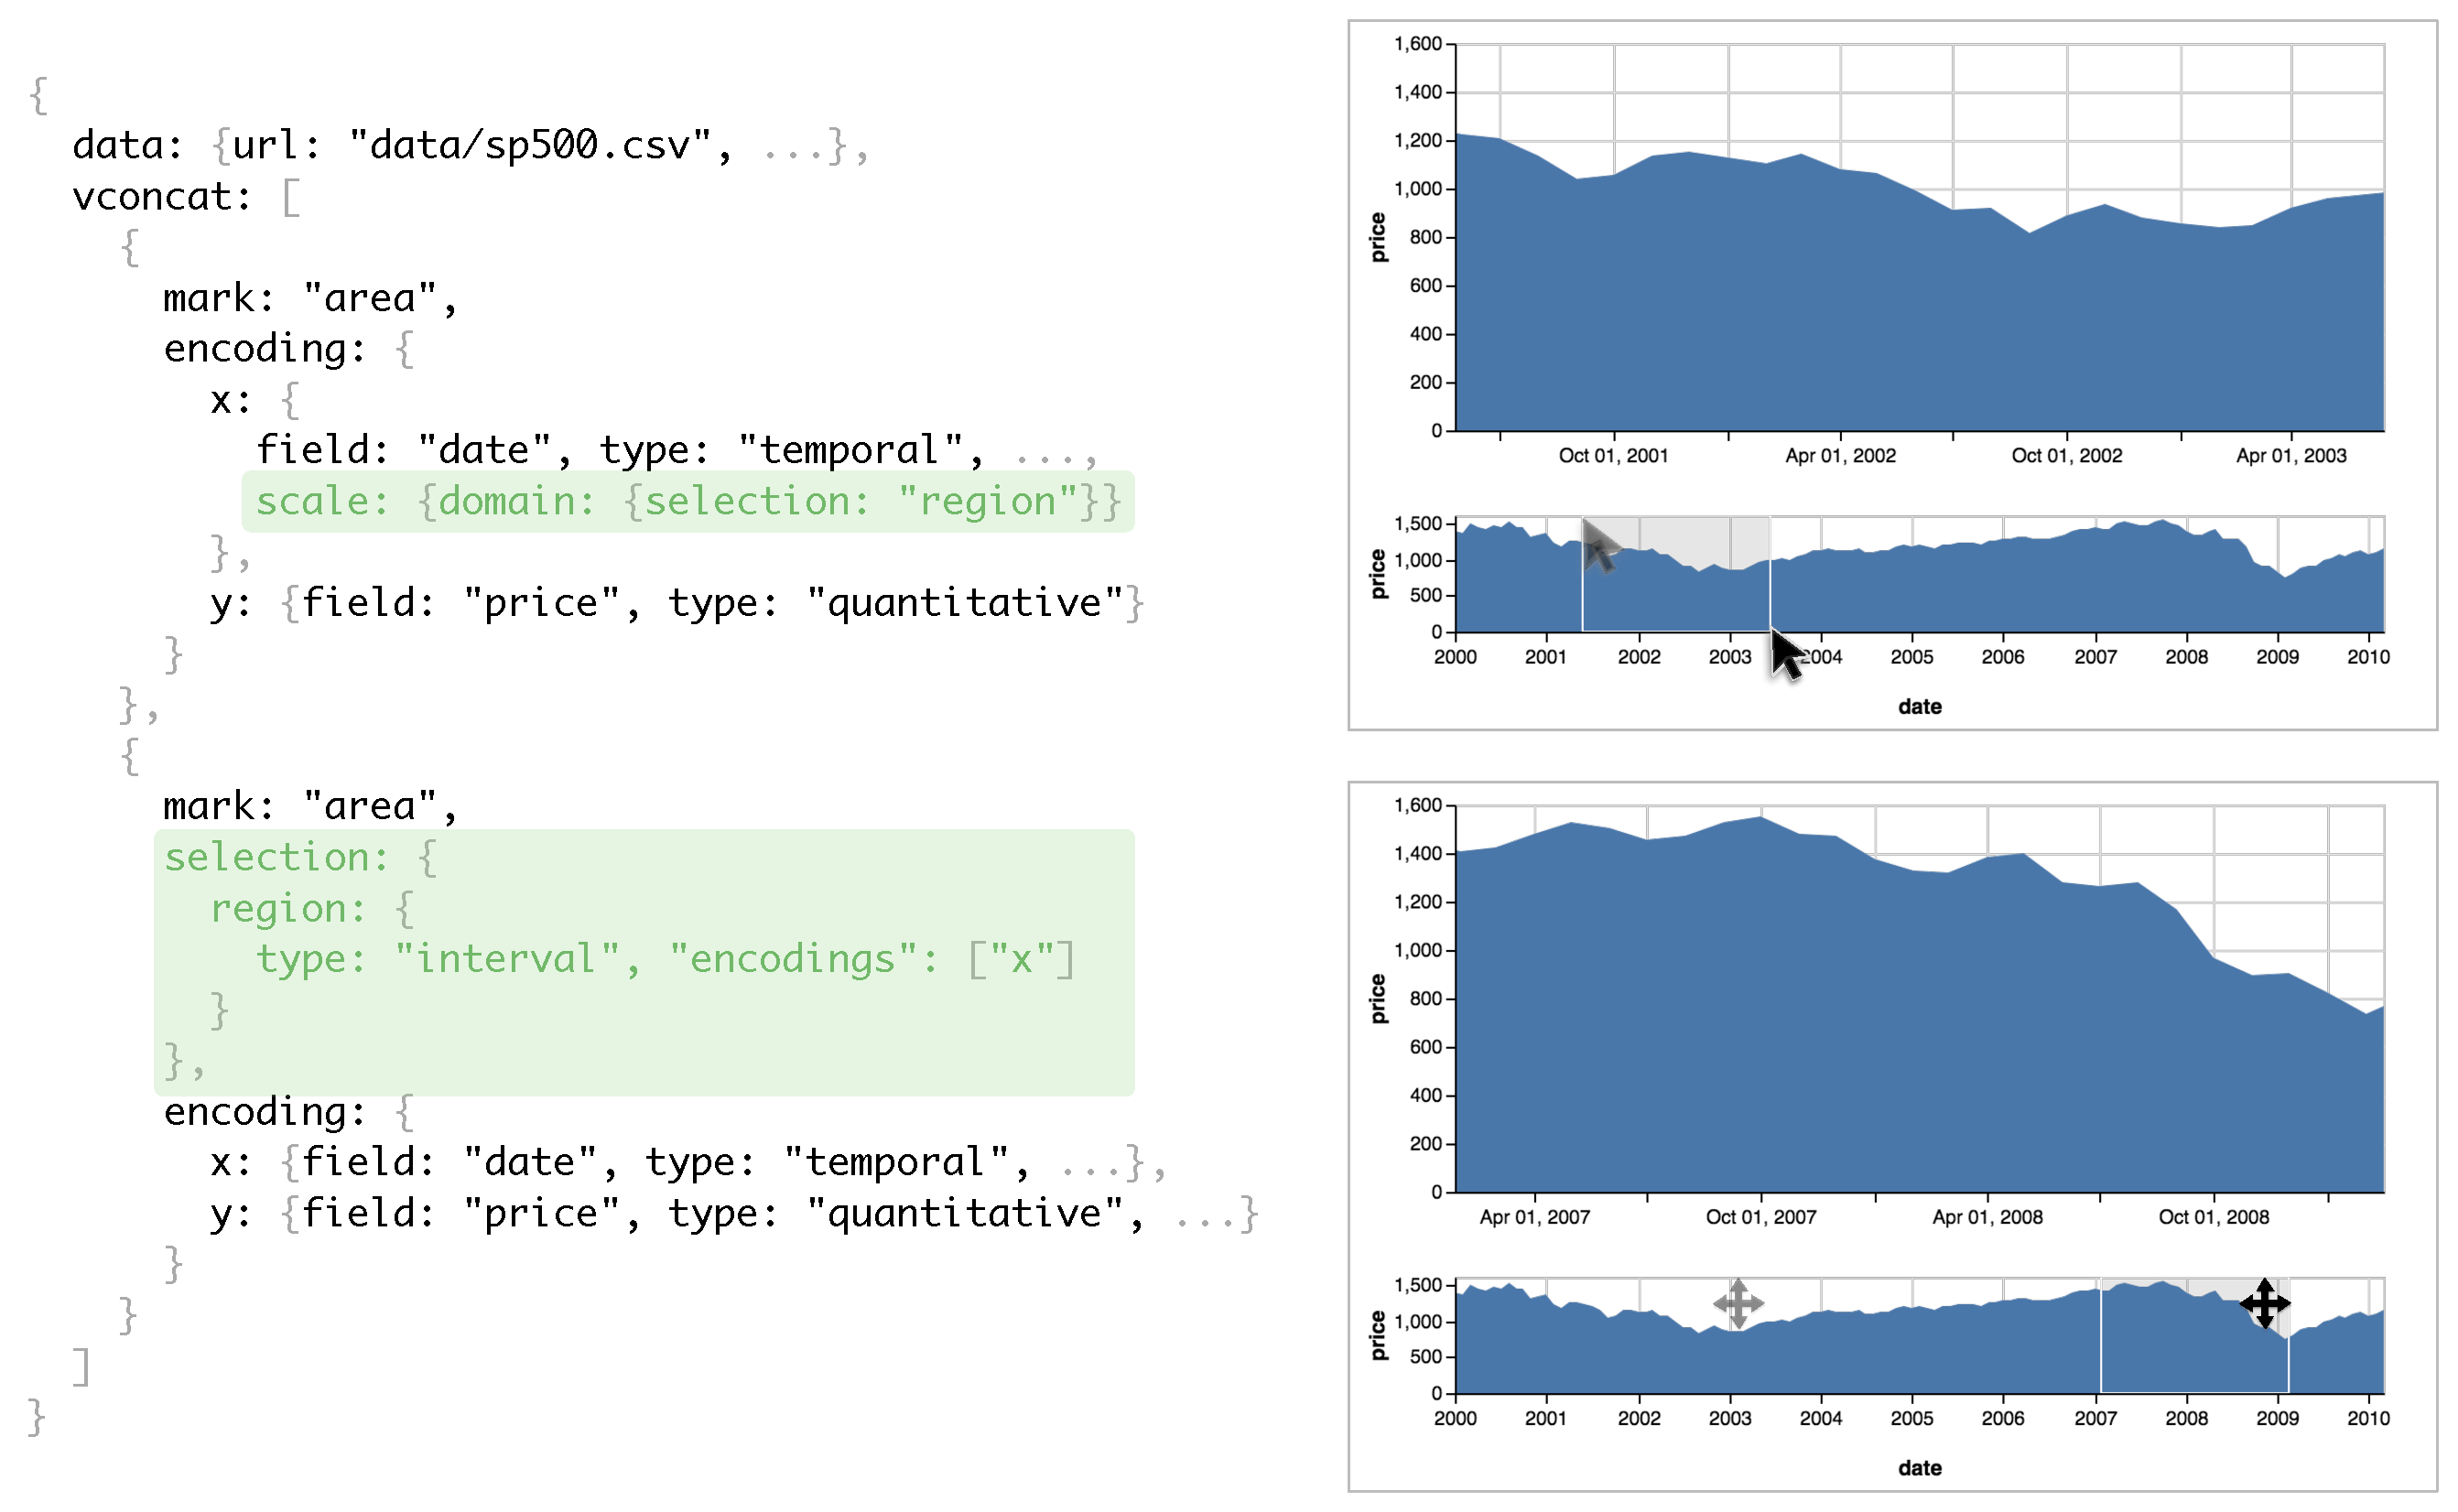
\includegraphics[width=\columnwidth]{overviewDetail}
  \caption{An overview\,+\,detail visualization concatenates two unit
  specifications, with a selection in the second one parameterizing the x-scale
  domain in the first.}
  \label{fig:vl:overviewDetail}
\end{figure}

\subsection{Reconfigure: Index Chart}

\Cref{fig:vl:indexChart} uses a single selection to interactively normalize
stock price time series data as the user moves their mouse across the chart. We
apply the \emph{nearest} transform to accelerate the selection using an
invisible Voronoi diagram. By projecting over the \texttt{date} field, the
selection represents both a single data value as well a set of values that share
the selected \texttt{date}. Thus, we can reference the single selection
directly, to position the red vertical rule, and also materialize it as part of
the \emph{lookup} data transform.

\begin{figure}[h!]
  \centering
  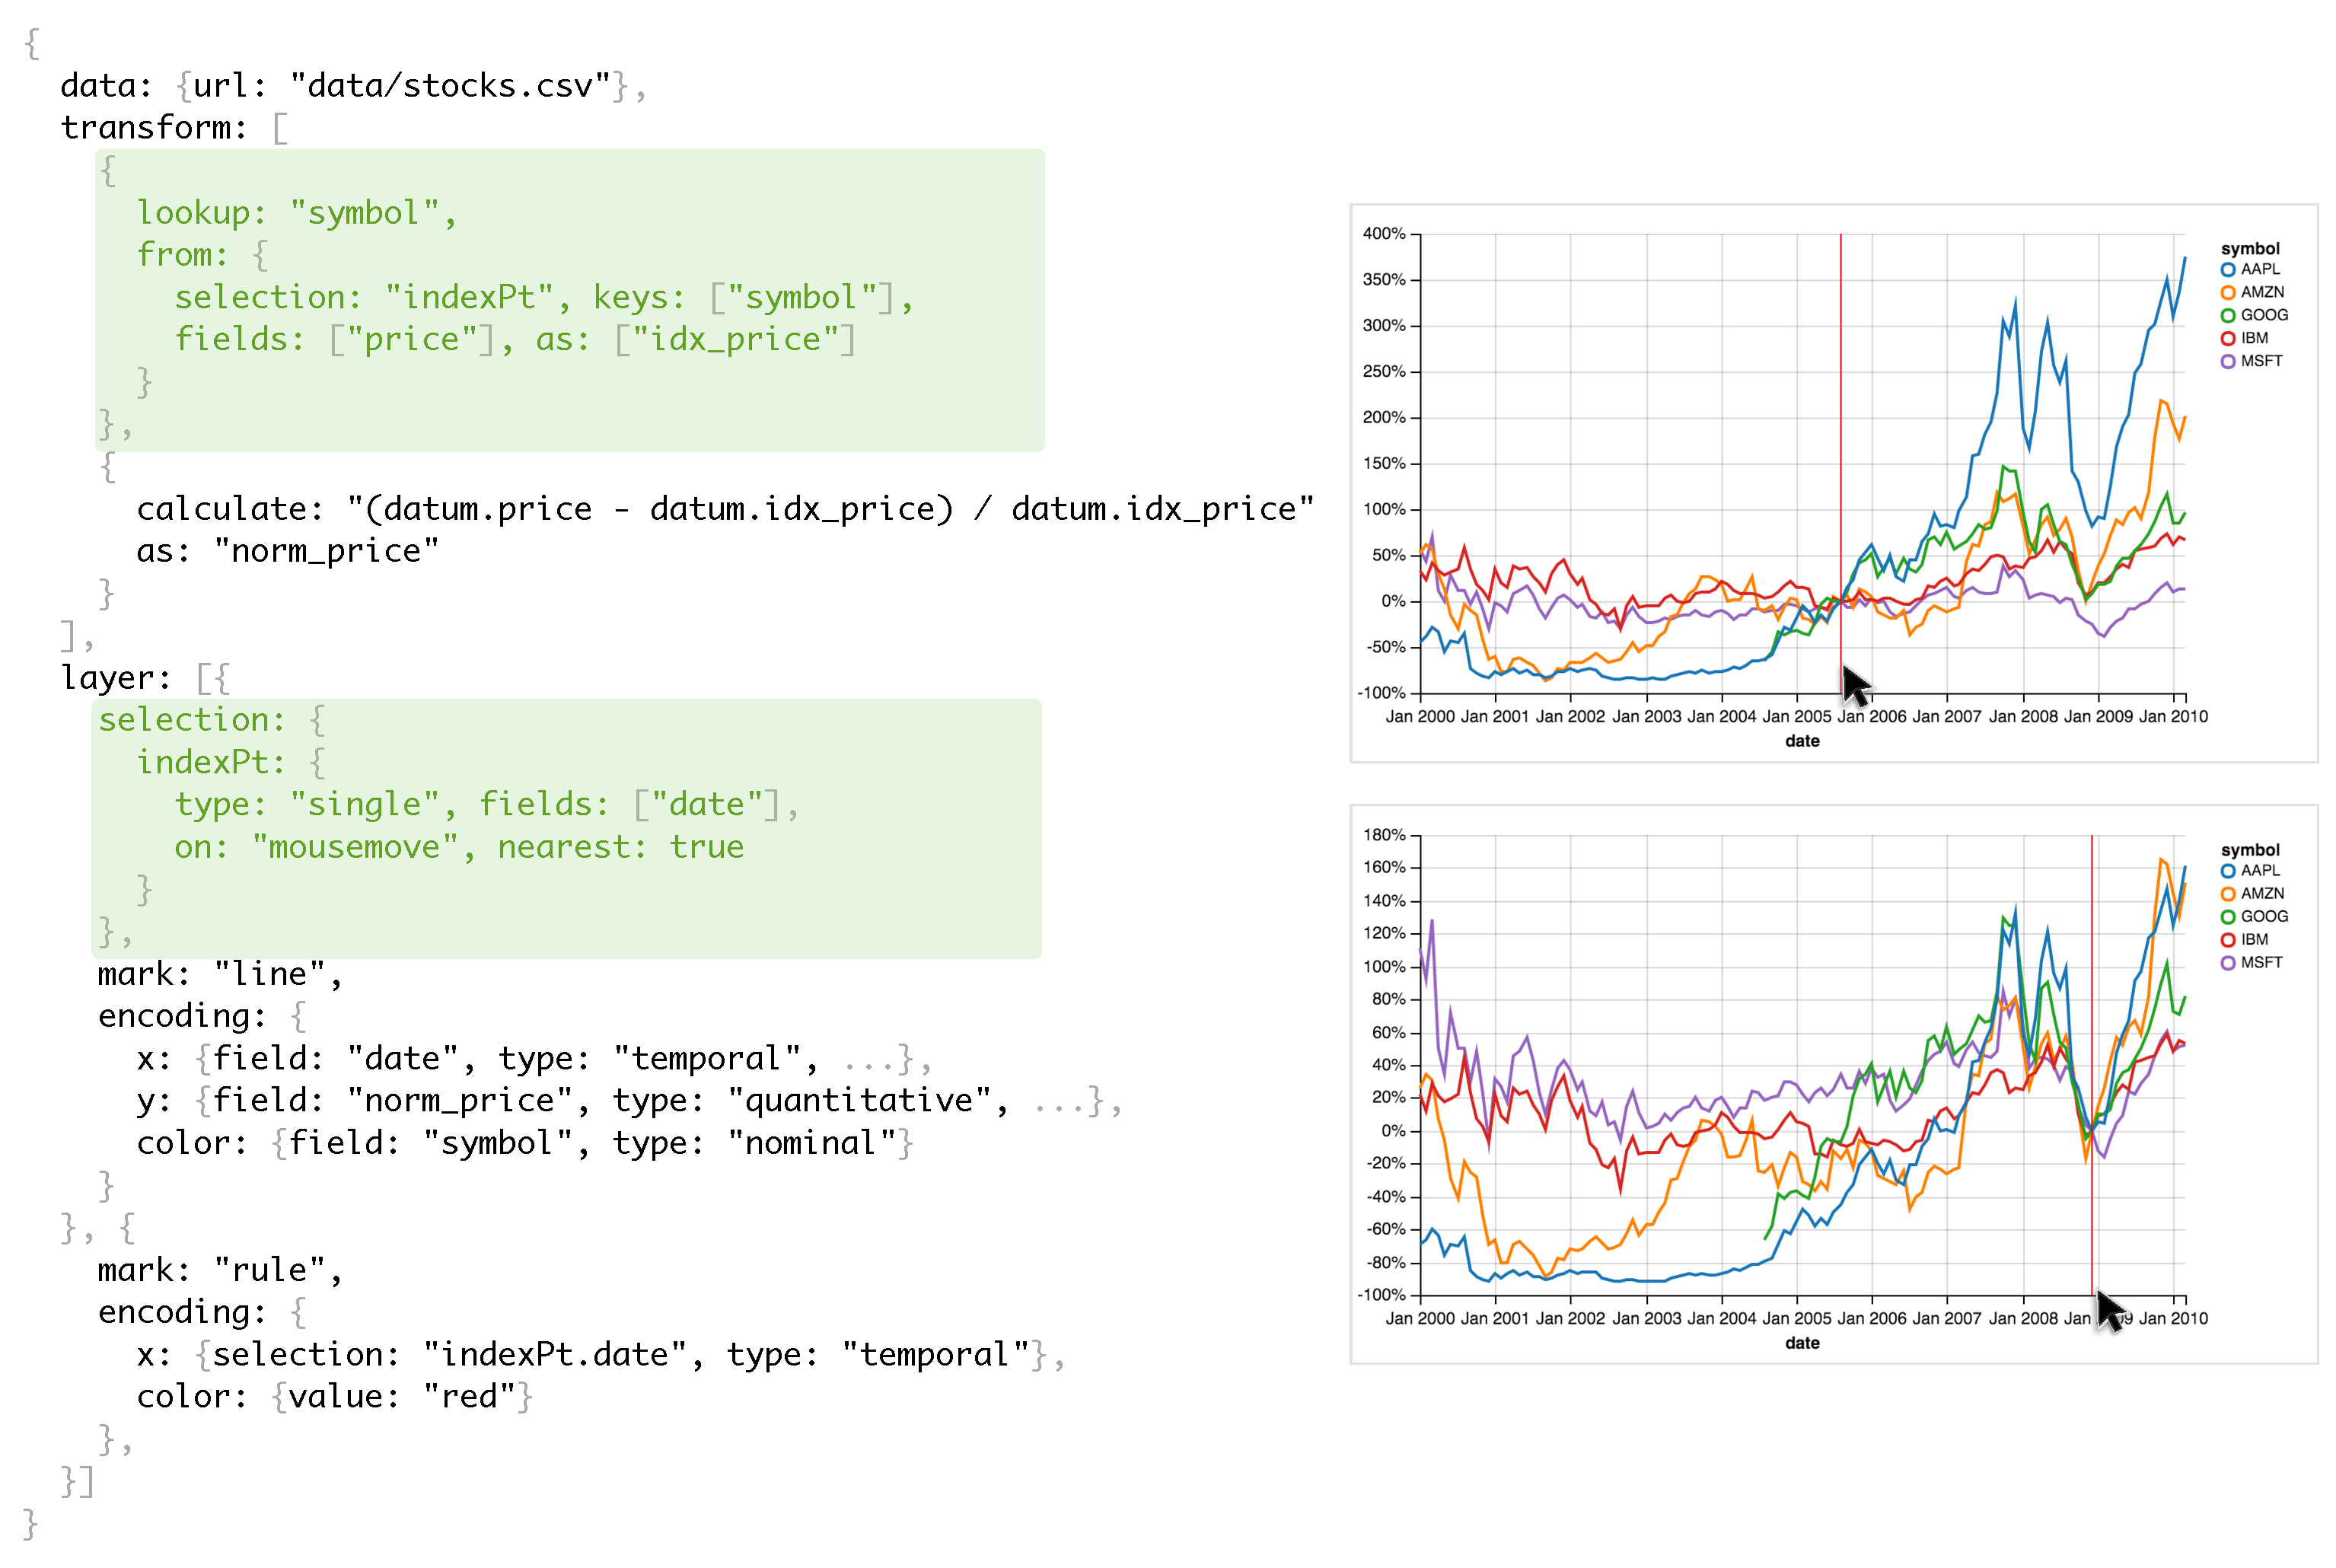
\includegraphics[width=\columnwidth]{indexChart}
  \caption{An index chart uses a single selection to renormalize data based
  on the index point nearest the mouse cursor.}
  \label{fig:vl:indexChart}
\end{figure}

\subsection{Filter: Cross Filtering}

As selections provide a predicate function, it is trivial to use them to filter
a dataset. \Cref{fig:vl:crossfilter}, for example, presents a concise
specification to enable filtering across three distinct binned histograms. It
uses a \emph{repeat} operator with a uni-dimensional interval selection over the
bins set to \emph{intersect others}. The \emph{filter} data transform applies
the selection against the backing datasets such that only data values that fall
within the selection are displayed. Thus, as the user brushes in one histogram,
the datasets that drive each of the other two are filtered, the data values are
re-aggregated, and the bars rise and fall. As with other interval selections,
the Vega-Lite compiler automatically instantiates the \emph{translate}
transform, allowing users to drag brushes around rather than having to reselect
them from scratch.

\begin{figure}[h!]
  \centering
  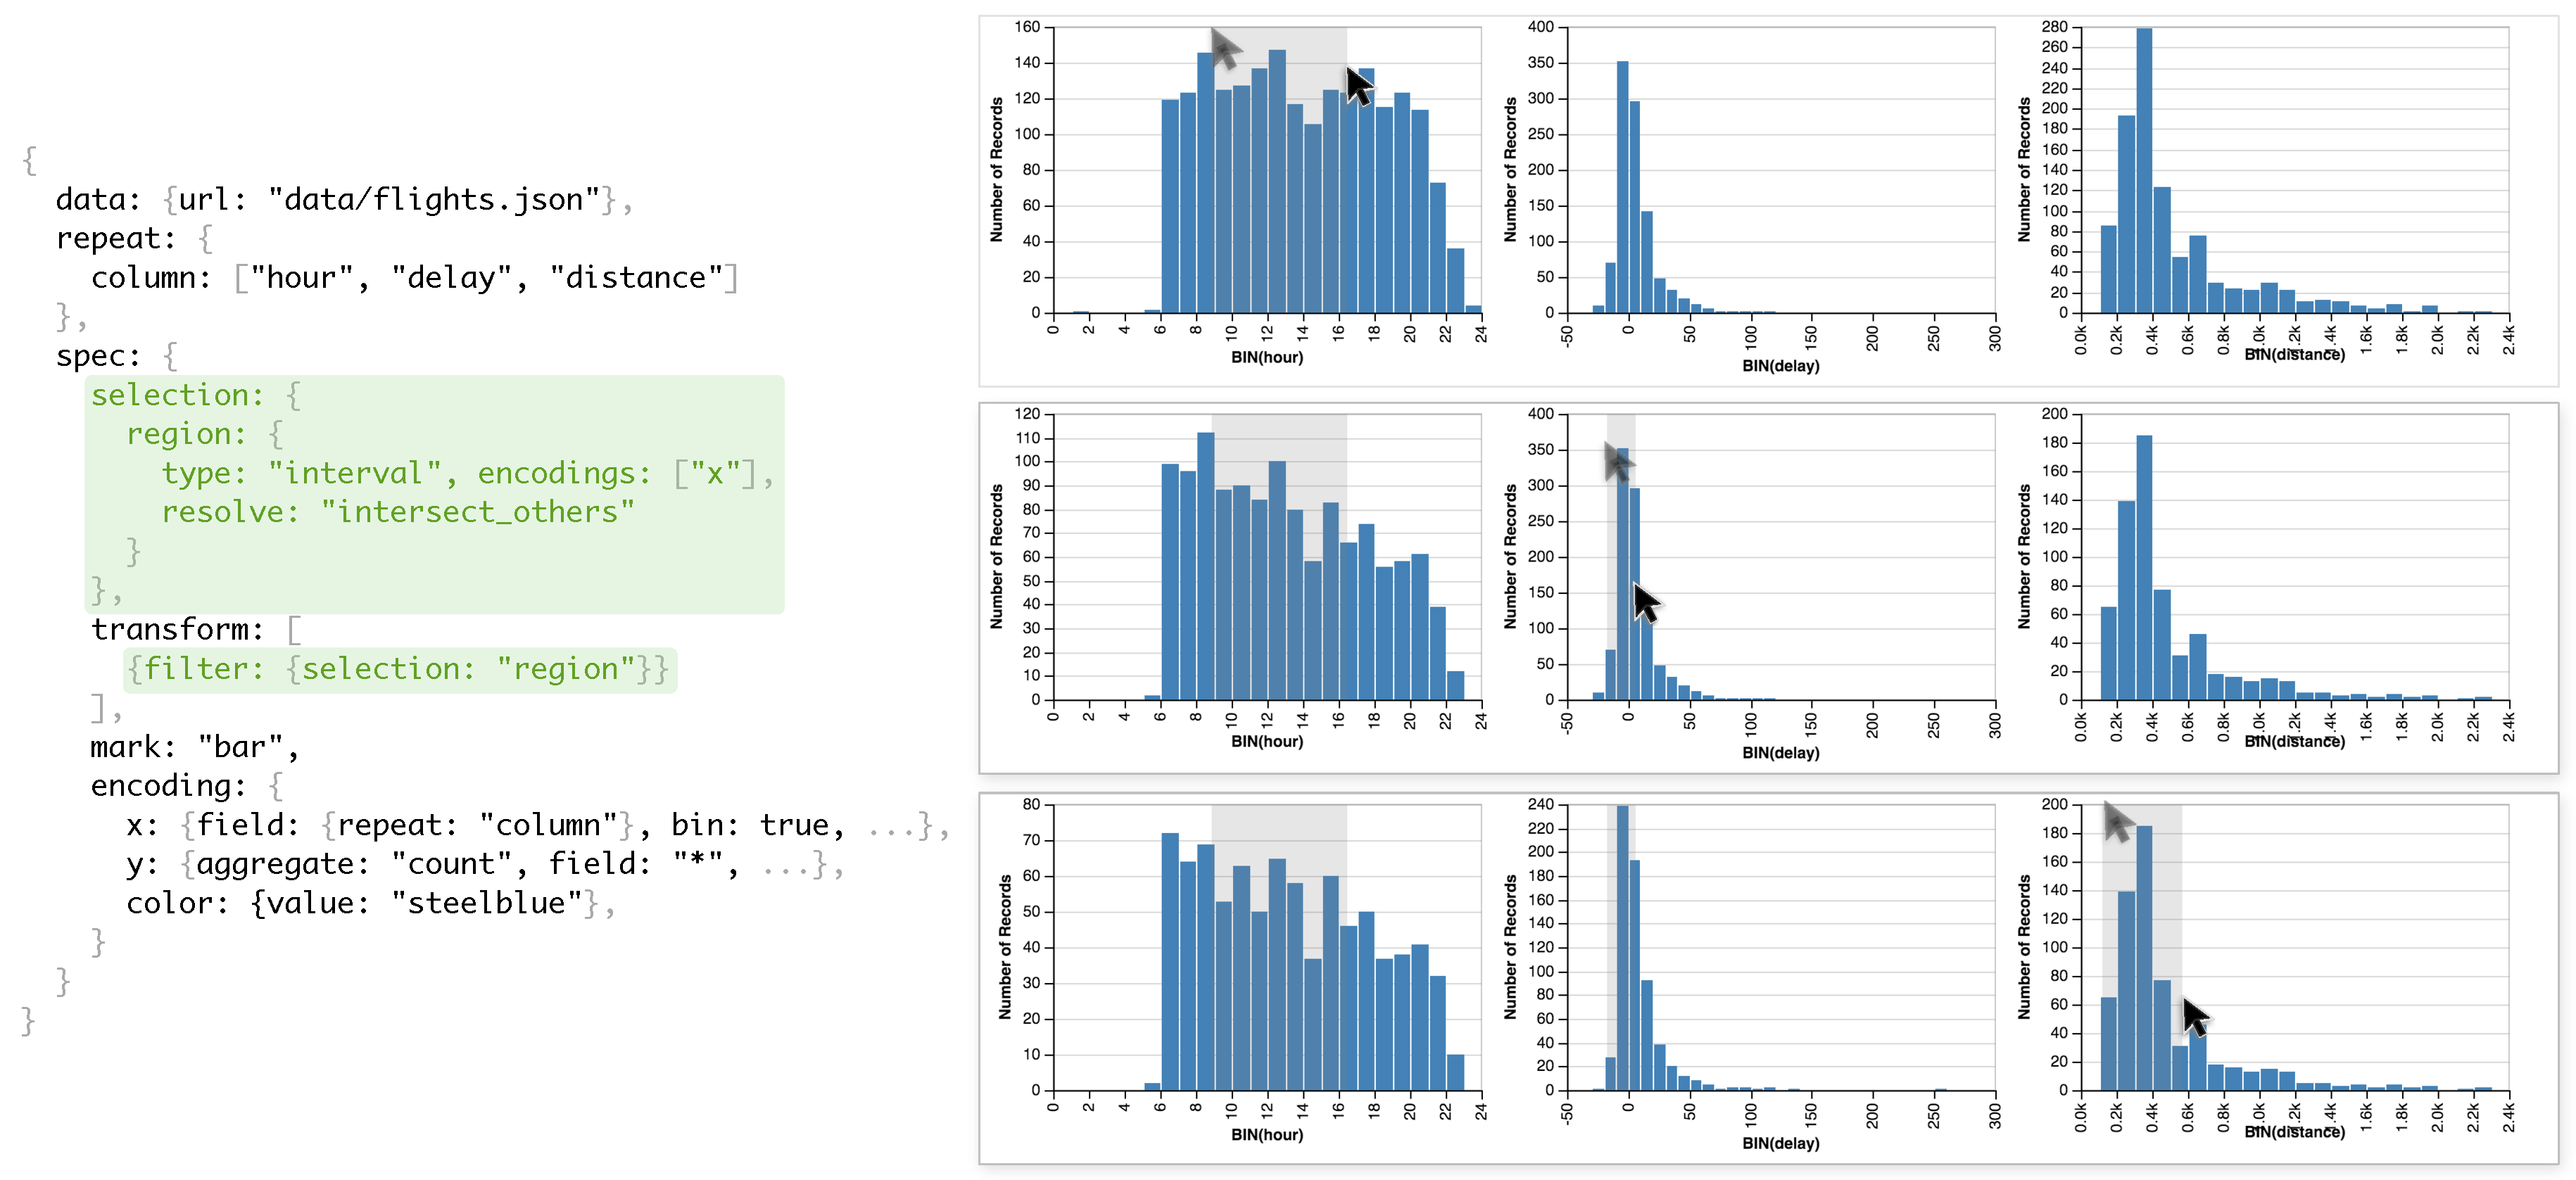
\includegraphics[width=\columnwidth]{crossfilter}
  \caption{An interval selection, resolved to \emph{intersect others}, drives a
  cross filtering interaction. Brushing in one histogram filters and
  reaggregates the data in the others, observable by the varying y-axis labels
  in the screenshots.}
  \label{fig:vl:crossfilter}
\end{figure}

The \emph{filter} data transform can also be used to materialize the selection
as an input dataset for secondary views. For instance, one drawback of
cross-filtering as in \cref{fig:vl:crossfilter} is that users only see the
selected values, and lose the context of the overall dataset. Instead of
applying the selection back onto the input dataset, we can instead materialize
it as an overlay (\cref{fig:vl:layeredCrossfilter}). Now, as the user brushes in
one histogram, bars highlight to visualize the proportion of the overall
distribution that falls within the brushed region(s). With this setup, it is
necessary to change the selection's resolution to simply \emph{intersect}, such
that bars in the brushed plot also highlight during the interaction.

\begin{figure}[h!]
  \centering
  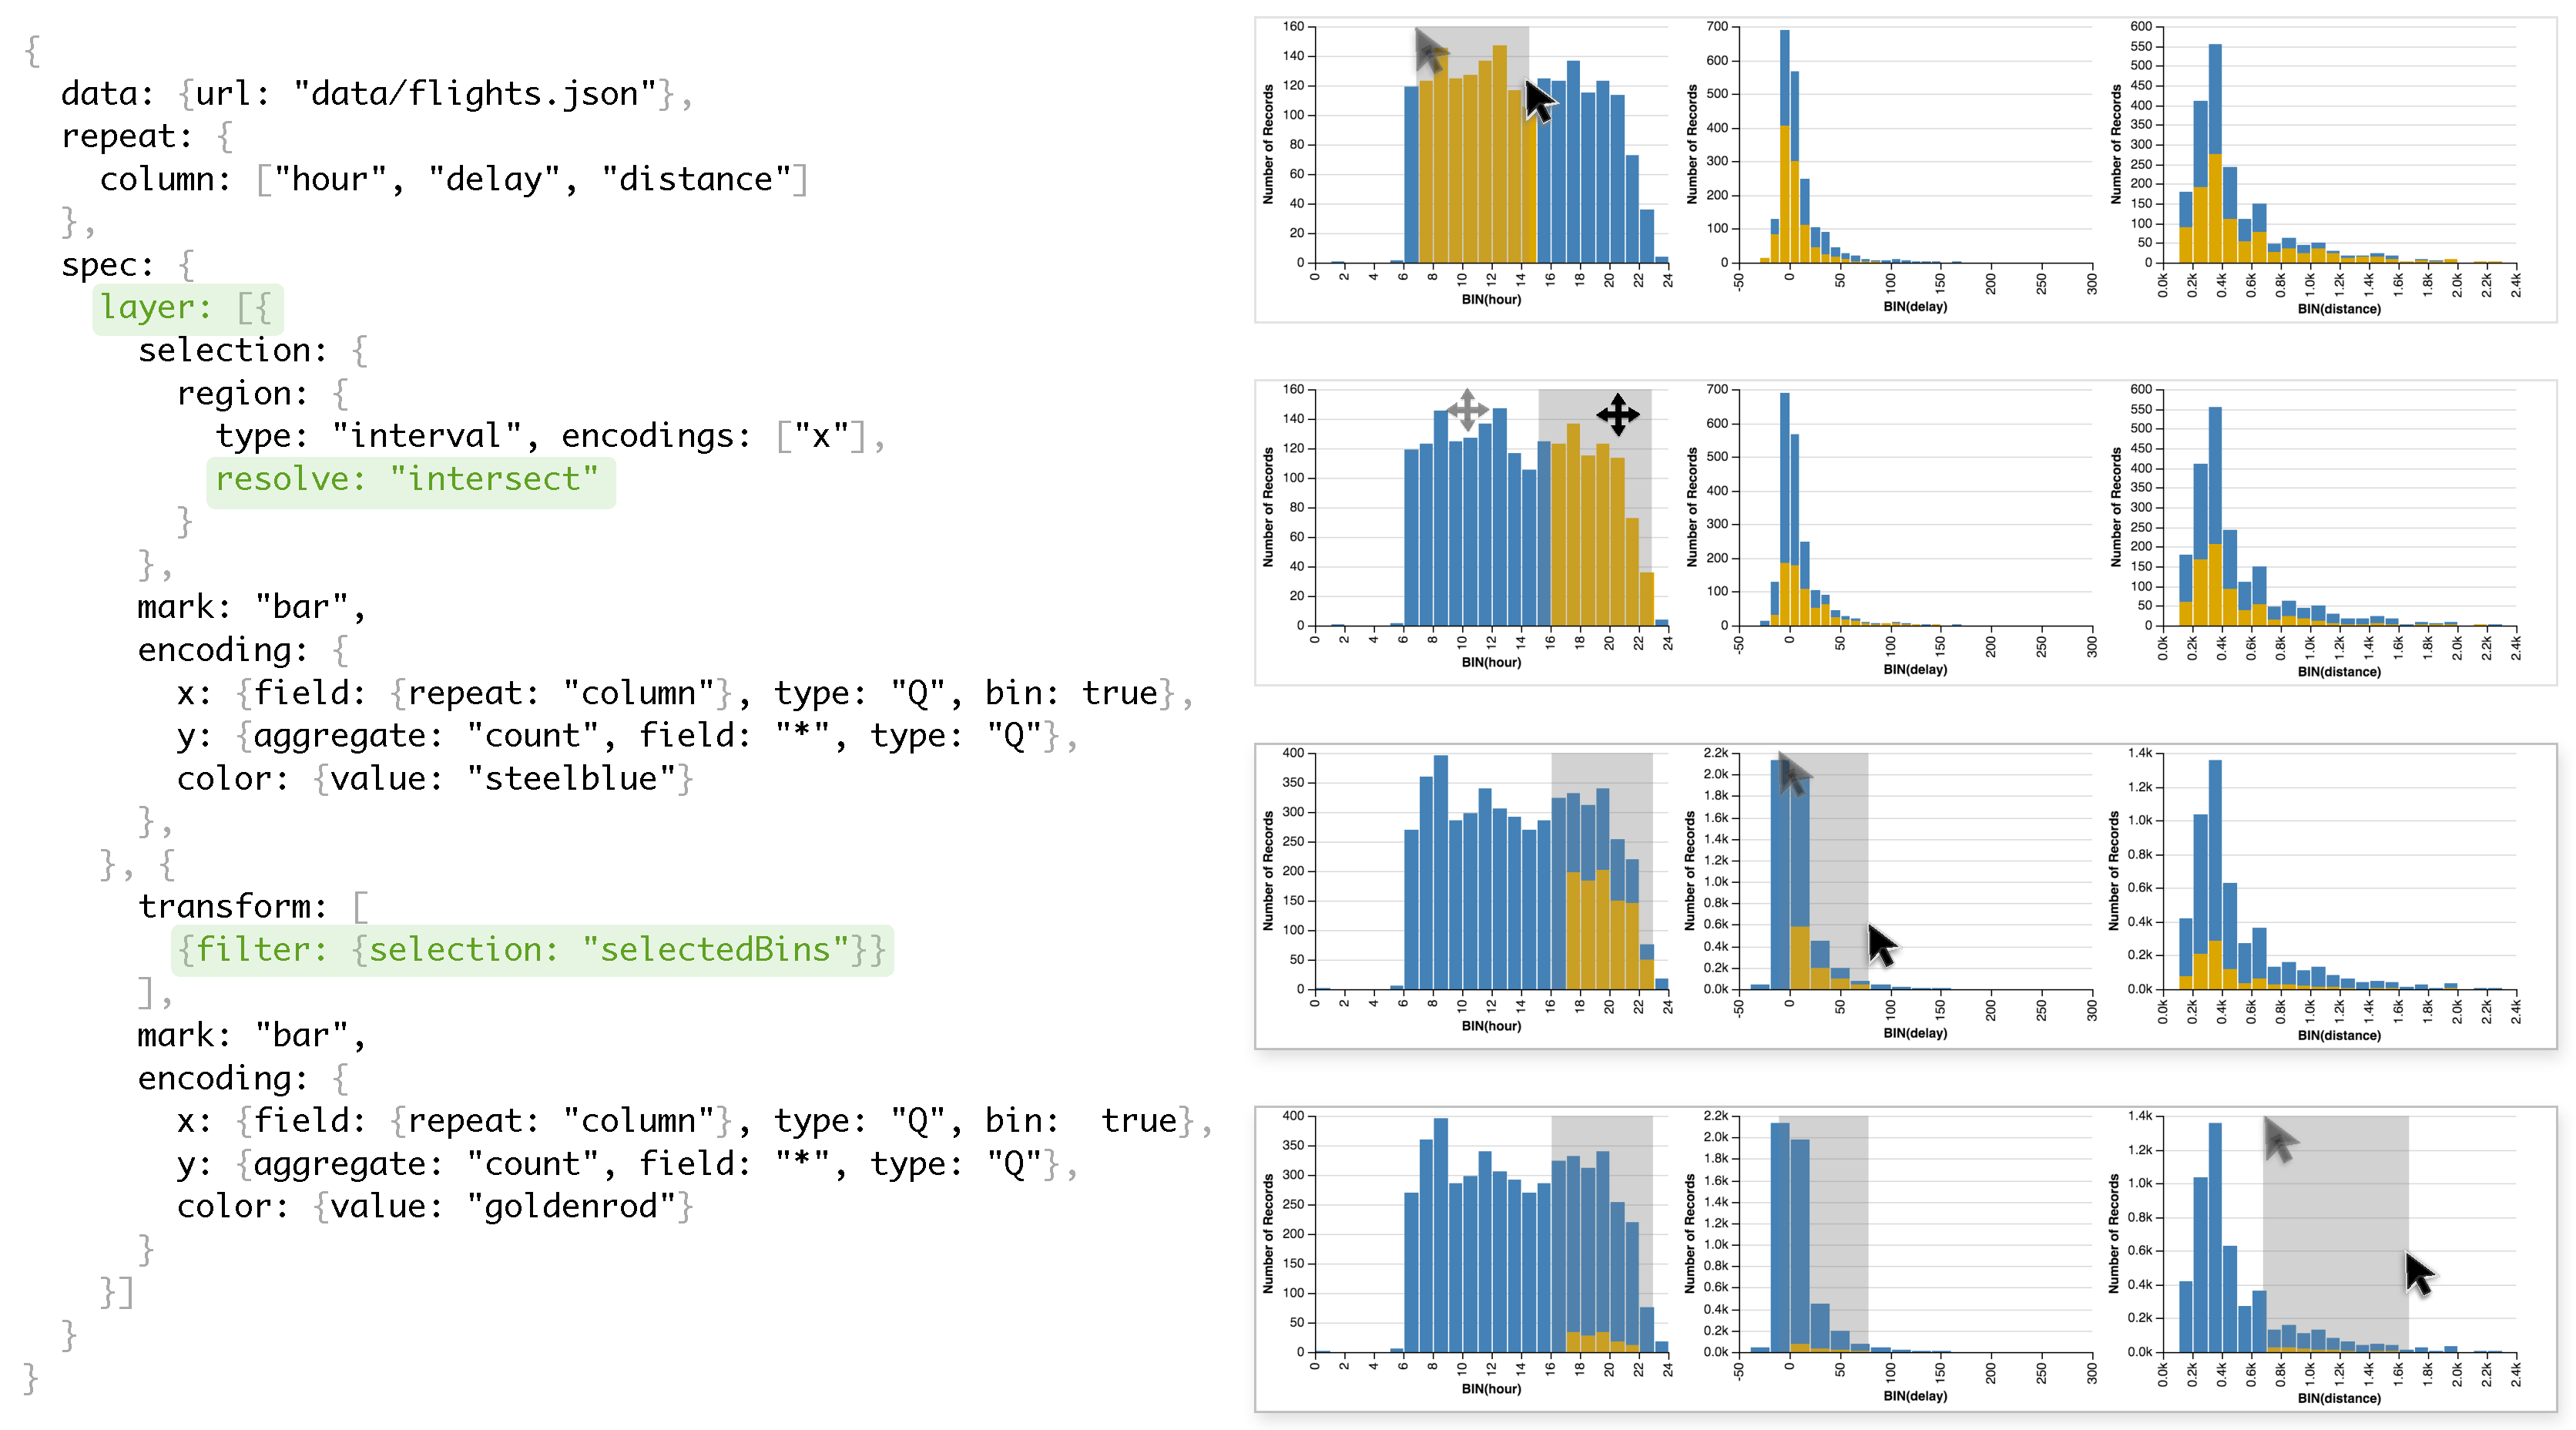
\includegraphics[width=\columnwidth]{layeredCrossfilter}
  \caption{A layered cross filtering interaction is constructed by resolving
  the interval selection to \emph{intersect}, and then materializing it to
  serve as the input data for a second layer. Highlights indicate changes to
  the specification from~\cref{fig:vl:crossfilter}.}
  \label{fig:vl:layeredCrossfilter}
\end{figure}

\subsection{Limitations}

The previous examples demonstrate that Vega-Lite specifications are more concise
than those of the lower-level Vega language, and yet are sufficiently expressive
to cover an interactive visualization taxonomy. Moreover, we have shown how
primitives can be systematically enumerated to facilitate exploration of
alternative designs. Nevertheless, we identify two classes of limitations that
currently exist.

First, there are limitations that are a result of how our formal model has been
reified in the current Vega-Lite implementation. In particular, components that
are determined at compile-time cannot be interactively manipulated. For example,
a selection cannot specify alternate fields to bin or aggregate over. Similarly,
more complex selection types (e.g., lasso selections) cannot be expressed as the
Vega-Lite system does not support arbitrary path marks. Such limitations can be
addressed with future versions of Vega-Lite, or alternate systems that
instantiate its grammar. For example, rather than a \emph{compiler},
interactions could parameterize the entirety of a specification within a
Vega-Lite \emph{interpreter}.

The second class of limitations are inherent to the model itself. As a
higher-level grammar, our model favors conciseness over expressivity. The
available primitives ensure that common methods can be rapidly specified, with
sufficient composition to enable more custom behaviors as well. However, highly
specialized techniques, such as querying time-series data via relaxed
selections~\cite{holz:relaxed}, cannot be expressed by default. Fortunately, our
formulation of selections, which decouple backing points from selected points
via a predicate function, provide a useful abstraction for extending our base
semantics with new, custom transforms. For example, the aforementioned technique
could be encapsulated in a \emph{relax} transform applicable to multi
selections.

While our selection abstraction supports \emph{interactive} linking of marks,
our view algebra does not yet provide means of \emph{visually} linking marks
across views (e.g., as in the Domino system~\cite{gratzl:domino}). Our view
algebra might be extended with support for connecting corresponding marks. For
example, points in repeated dot plots could be visually linked using line
segments to produce a parallel coordinates display.
% !TEX root = ../thesis.tex
\section{Limitations \& Future Work}
\label{sec:vl:conclusion}

The previous section demonstrates that Vega-Lite specifications are more concise
than those of the lower-level Vega language, and yet are sufficiently expressive
to cover an interactive visualization taxonomy. Moreover, we have shown how
primitives can be systematically enumerated to facilitate exploration of
alternative designs. Nevertheless, we identify two classes of limitations that
currently exist.

First, there are limitations that are a result of how our formal model has been
reified in the current Vega-Lite implementation. In particular, components that
are determined at compile-time cannot be interactively manipulated. For example,
a selection cannot specify alternate fields to bin or aggregate over. Similarly,
more complex selection types (e.g., lasso selections) cannot be expressed as the
Vega-Lite system does not support arbitrary path marks. Such limitations can be
addressed with future versions of Vega-Lite, or alternate systems that
instantiate its grammar. For example, rather than a \emph{compiler},
interactions could parameterize the entirety of a specification within a
Vega-Lite \emph{interpreter}.

The second class of limitations are inherent to the model itself. As a
higher-level grammar, our model favors conciseness over expressivity. The
available primitives ensure that common methods can be rapidly specified, with
sufficient composition to enable more custom behaviors as well. However, highly
specialized techniques, such as querying time-series data via relaxed
selections~\cite{holz:relaxed}, cannot be expressed by default. Fortunately, our
formulation of selections, which decouple backing points from selected points
via a predicate function, provide a useful abstraction for extending our base
semantics with new, custom transforms. For example, the aforementioned technique
could be encapsulated in a \emph{relax} transform applicable to list selections.

While our selection abstraction supports \emph{interactive} linking of marks,
our view algebra does not yet provide means of \emph{visually} linking marks
across views (e.g., as in the Domino system~\cite{gratzl:domino}). Our view
algebra might be extended with support for connecting corresponding marks. For
example, points in repeated dot plots could be visually linked using line
segments to produce a parallel coordinates display.

An early version of Vega-Lite is used to automatically recommend static plots as
part of the Voyager browser~\cite{voyager}. Voyager leverages perceptual
\emph{effectiveness criteria}~\cite{bertin:semiology, cleveland:perception,
mackinlay:apt} to rank candidate visual encodings. One promising avenue for
future work is to develop models and techniques to analogously recommend
suitable interaction methods for given visualizations and underlying data types.
Here, the human-computer interaction literature~\cite{beaudouin:instrumental}
may offer insights on when and why users benefit from certain interaction
techniques.

Vega-Lite is an open source system available at
\url{http://vega.github.io/vega-lite/}. By offering a multi-view grammar of
graphics tightly integrated with a grammar of interaction, Vega-Lite facilitates
rapid exploration of design variations. Ultimately, we hope that it enables
analysts to produce and modify interactive graphics with the same ease with
which they currently construct static plots.